\chapter{Literature}
\label{background}
This chapter will first look at some general aspects of automated marking systems which already exist, and may give insight into how to improve the feedback of Infandango. The way the feedback is displayed defines what information is displayed to the student and so there will be discussion of how to visualise the feedback. The area of Cognitive Modelling will be discussed because it has had work performed to specifically give better feedback to students that use automated marking systems. The final piece of literature that will be discussed is about a system which is particularly similar to Infandango and which, recently, changed their method of feedback.

\section{Automated Marking Systems}
There are many other systems like Infandango and covering all of them in this report would be excessive. The systems which are discussed exemplify certain aspects of automated marking systems which are worth discussing with respect to Infandango. By looking at these systems and comparing the different forms of feedback they give it is hoped that weaknesses and potential improvements to Infandango's feedback system can be identified.

These systems are being discussed primarily for their marking and feedback methods, thus the other details of implementation will be largely ignored, but some form of code submission can be assumed for all these systems.

\subsection{RoboProf}
RoboProf\cite{roboprof} provides small programming exercises which start simple and get progressively harder, with immediate feedback about the correctness of the program guiding the student. For example, a student may be provided with a program which loops over a range of numbers and prints them. The student may then be asked to modify the for-loop in order to print out a different series of numbers. The immediate feedback gives the students encouragement and motivates them to keep trying more questions. This approach is similar to Infandango because both systems return immediate feedback based purely on the correctness of the output of the problem, and this is a common approach in other systems too\cite{webtoteach}.

In the paper one problem is identified: the immediate feedback is sometimes too addictive, and the students may end up spending more time than is necessary performing the exercises.

\subsection{Automated Evaluation of Programming Assignments}
Kaushal and Singh describe various measures used as part of an automated marking system: regularity, integrity, efficiency and accuracy\cite{automate_evaluation}. 
\begin{description}
\item[Regularity] The time at which a submission is made with respect to the deadline for that submission
\item[Integrity] The originality of the document determined through a plagiarism detector
\item[Efficiency] A qualitative measure of the time taken and memory used by a student's programs
\item[Accuracy] The percentage of test cases for each program that the student's submission passes
\end{description}

The experimenters track the change in these measures as students use the system and find that there is a general improvement on all categories when feedback is based on these measurements. There are other systems which use similar measures of feedback\cite{ASSYST} and this automated feedback has be shown to be at least as good as manual feedback\cite{coursemaster}.

One disadvantage of having different measures for feedback is that this still requires manual work in the specification of the feedback. For example, the ASSYST system\cite{ASSYST} uses a metric first proposed by Berry and Meekings\cite{berrymeekings} to measure the style of the submitted programs. This means tutors must specify four values which create a simple graph which determines the mark a student receives based on their style score. The specific details can be found in the paper, but what it means is that each time a new measurement is to be used for a new feedback measure, then a new metric system must be implemented as well as the measurement itself. A system in which the measurement itself is enough, and the rest of the process is automated, would be an improvment.

\section{Visualisation}
In his book {\it Visual Display of Quantitative Information}\cite{visual_explanations}, Edward Tufte discusses methods of efficiently and effectively displaying information. In Chapter 4 ``Data-Ink and Graphical Redesign'', Tufte introduces the idea of Data-Ink: The amount of ``ink'' which is actually used to represent the data you are interested in. In Tufte's words:

\begin{quote}Data-ink is the non-erasable core of a graphic, the non-redundant ink arranged in reponse to the variation in the numbers represented.
\end{quote}
Data-ink is desirable, unavoidable information so Tufte says designers should strive towards a high data-ink ratio, removing as much non-information ink as possible to avoid overwhelming the data. Tufte then continues by giving examples where redundant information is desirable. One of these examples uses a graphic from Linus Pauling's General Chemistry\cite{general_chemistry}. Figure \ref{fig:tuftegraphs} shows how, based on the low data-ink ratio principle, Tufte removes the grid marks and part of the frame which leaves little else but the data itself.

\begin{figure}[h!]
\centering
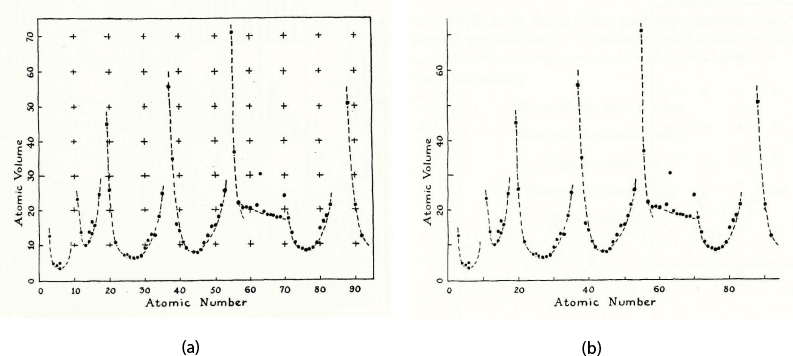
\includegraphics[width=0.8\textwidth]{images/tuftegraphs.png}
\caption{(a) shows the original graph and (b) shows how Tufte recommends changing the graph to remove redundant information}
\label{fig:tuftegraphs}
\end{figure}


Tufte concludes the chapter with 5 maxims summarising this principle.

\begin{verse}
	Above all else show the data.
	
	Maximize the data-ink ratio.
	
	Erase non-data-ink.
	
	Erase redundant data-ink.
	
	Revise and edit.
	
\end{verse}

Infandango currently adheres to these principles quite well. For example, the score which is provided for each question is displayed as a percentage on a block of colour, which is dependent on the score. At first the block of colour may seem redundant since it is a feature related directly to the score so it doesn't seem to add much information. However, the score alone would not tell the user if that score is ``good'' or ``bad'', that is a judgement the user would have to make for themselves. Providing this information as a colour is a simple, intuitive way of telling the use whether their performance on an exercise is acceptable or not.

\section{Cognitive Modelling}
The cognitive modelling of students can provide access to important information for automatic tutoring systems. A cognitive model is a computer model of the cognitive processes of a student, which allows insight into how the student might approach the problem, or how difficult the problem might be for the student. Building this model manually requires a lot of human effort\cite{simstudent_better} and so automating this process is desirable.

SimStudent is a machine learning agent designed to build cognitive models automatically via machine learning. The machine learning method used for parts of SimStudent is a First Order Inductive Learner, which is given some some observations and background knowledge from which it draws hypotheses. Using algebra as an example, SimStudent will be given some basic operators as background knowledge (add, subtract, multiply, divide) and will then be given an algebraic problem to solve. It will then suggest the next step to the student who may reject or accept the suggestion, thus providing negative or positive feedback to SimStudent to modify its production rules.

As long as the students perform consistently, SimStudent can model the performance of the students with an accuracy of 83\%\cite{simstudent}. Being able to model and predict a student's performance can allow the tutoring system to target feedback at the areas which it knows the student might struggle with, thus catching problems before they occur and understanding why certain mistakes happen. This research shows that machine learning can be used to generate feedback which is better or equivalent to manual feedback.

\section{Machine Learning and Feedback for an Online Marking System}
Khan Academy\cite{khan_site} is a website which provides users with online education material:
\begin{quote}
Our online materials cover subjects ranging from math and finance to history and art.  With thousands of bite-sized videos, step-by-step problems and instant data\cite{ka_faq}
\end{quote}

\begin{figure}[h!]
\centering
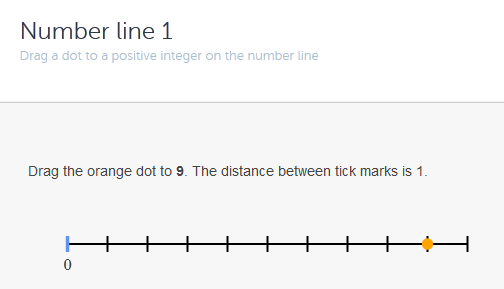
\includegraphics[width=0.8\textwidth]{images/kascreenshot.png}
\caption{A screenshot of the online Khan Academy system, showing a simple exercise where the user must choose the correct position on a number line.}
\label{fig:kascreenshot}
\end{figure}

A blog post\cite{khan_blog} written by David Hu about Khan Academy explains how they went about changing their feedback system. Khan Academy gives users certain kinds of exercises, for example choosing the approriate position on a number scale (see Figure \ref{fig:kascreenshot}). It can then generate endless variations of this problem for the user to continue attempting until they are deemed proficient. Proficiency is the phrase used by Khan Academy when it judges the user to be good enough at a certain type of exercise that the user should move on. The original Khan Academy system required the user to get 10 consecutive exercises of a certain type correct (a ``streak'') before they are qualified as proficient for that type of exercise. 

The main problem with this system is that a user could get 9 consecutive exercises correct and then make a mistake on the final exercise. Before the user could move on they would have to get 10 more consecutive exercises correct. Hu decided to search for a new system which would be less fickle, thus removing some of the frustration experienced by students.

In an attempt to improve this system, Hu proposed using a logistic regression model to calculate the probability that a user passes the next exercise successfully, with a threshold of 94\% representing the new proficiency level. To explain a logistic regression it helps to have some terminology. 

\begin{description}
\item[features] The observed data which will be used to make a prediction, e.g. the mark for the previous submission
\item[weights] A constant multiplier applied to the features. The higher the weight, the more that feature contributes to the prediction
\end{description}

The logistic regression is quite simple: it applies the weights to the features and sums the results to get a single value. In order to turn this value into a probability it must be squashed into the range 0, 1. The function used to do this is the logistic function, where x is the value you want to squash into the range 0, 1:

\begin{displaymath}
\frac{1}{1+e^{-x}}
\end{displaymath}

Over a 6 day period 10\% of users tested the new method. Users of the new system earned 20.8\% more proficiences, attempted 15.7\% more exercises and required 26\% less exercises per proficiency. Hu summarises by saying the boost seems to come from allowing users to move on from exercises which they are already proficient at, without requiring them to complete their streak.

Although the current Infandango system does not require perfection like Khan Academy did, it is possible that users are more reluctant to move on from exercises before they achieve 100\% because with the marking done automatically with objective tests it is possible and common to get 100\% for exercises. Encouraging the user to move on when they do not yet have 100\% could encourage students to tackle more difficult problems.

This feedback is also interesting because it provides feedback across multiple exercises at the same time, but Infandango only marks individual exercises. Adapting the Khan Academy approach to provide summary feedback over multiple exercises gives the student an idea of their global progress.


\section{Conclusion}
The review of other automated marking systems shows us that there are other forms of feedback --- not just correctness of code --- which can be used in such systems. However, the current implementations still require some manual specification about how the measurement is translated into student feedback. A method of feedback which automatically translated measurements into feedback would be an interesting addition to Infandango.

The literature provides a strong case for applying machine learning to the problem of improving automated feedback. Infandango currently lacks feedback which uses information from multiple exercises, and having such feedback may allow more detailed and targeted feedback. While cognitive modelling is effective, it is more suited to rule based learning, where logic can be applied to the knowledge in order to learn hypotheses. The Khan Academy approach is more applicable to Infandango as it only needs to know the mark for an exercise, not the rules which a student applies in order to solve the exercise.
